\begin{figure}[!b]
\small
\centering
\resizebox{1\linewidth}{!}{
\begin{tabular}{|p{\linewidth}|} \hline
\begin{minipage}{\linewidth}
\vspace{0.1cm}
\small
{\bf \fig{xtree}.A: Using XTREE}

Using the training data, construct a decision tree. For each test item, find the {\em current} leaf: take each test instance, run it down to a leaf in the decision tree.  
After that,	find the {\em desired} leaf:
\begin{itemize}[leftmargin=3mm]
\item Starting at {\em current}, ascend the tree levels;
\item Identify {\em sibling} leaves; i.e. leaf clusters that can be reached from level $lvl$ that are not same as {\em current}
\item Find the {\em better} siblings; i.e. those with a {\em score} (\#defects) less than $\gamma=0.5$ times the score of {\em current} branch. 
If none found, then repeat for $lvl += 1$. Also, return no plan if the new $lvl$ is above the root. 
\item  Return the {\em closest} better sibling to the {\em current}.
\end{itemize}
Also, find the {\em delta}; i.e. the set difference between conditions in the decision tree branch to {\em desired} and {\em current}. To find that delta: (1)~for discrete attributes, delta is the value from {\em desired}; (2)~for  numerics, delta is the numeric difference; (3)~for numerics  discretized into ranges, delta is a random number selected from the low and high boundaries of the that range. Finally, return the delta as the plan for improving the test instance.\\
\end{minipage}
\begin{minipage}{\linewidth}
\textbf{\fig{xtree}.B: A sample decision tree.\\}
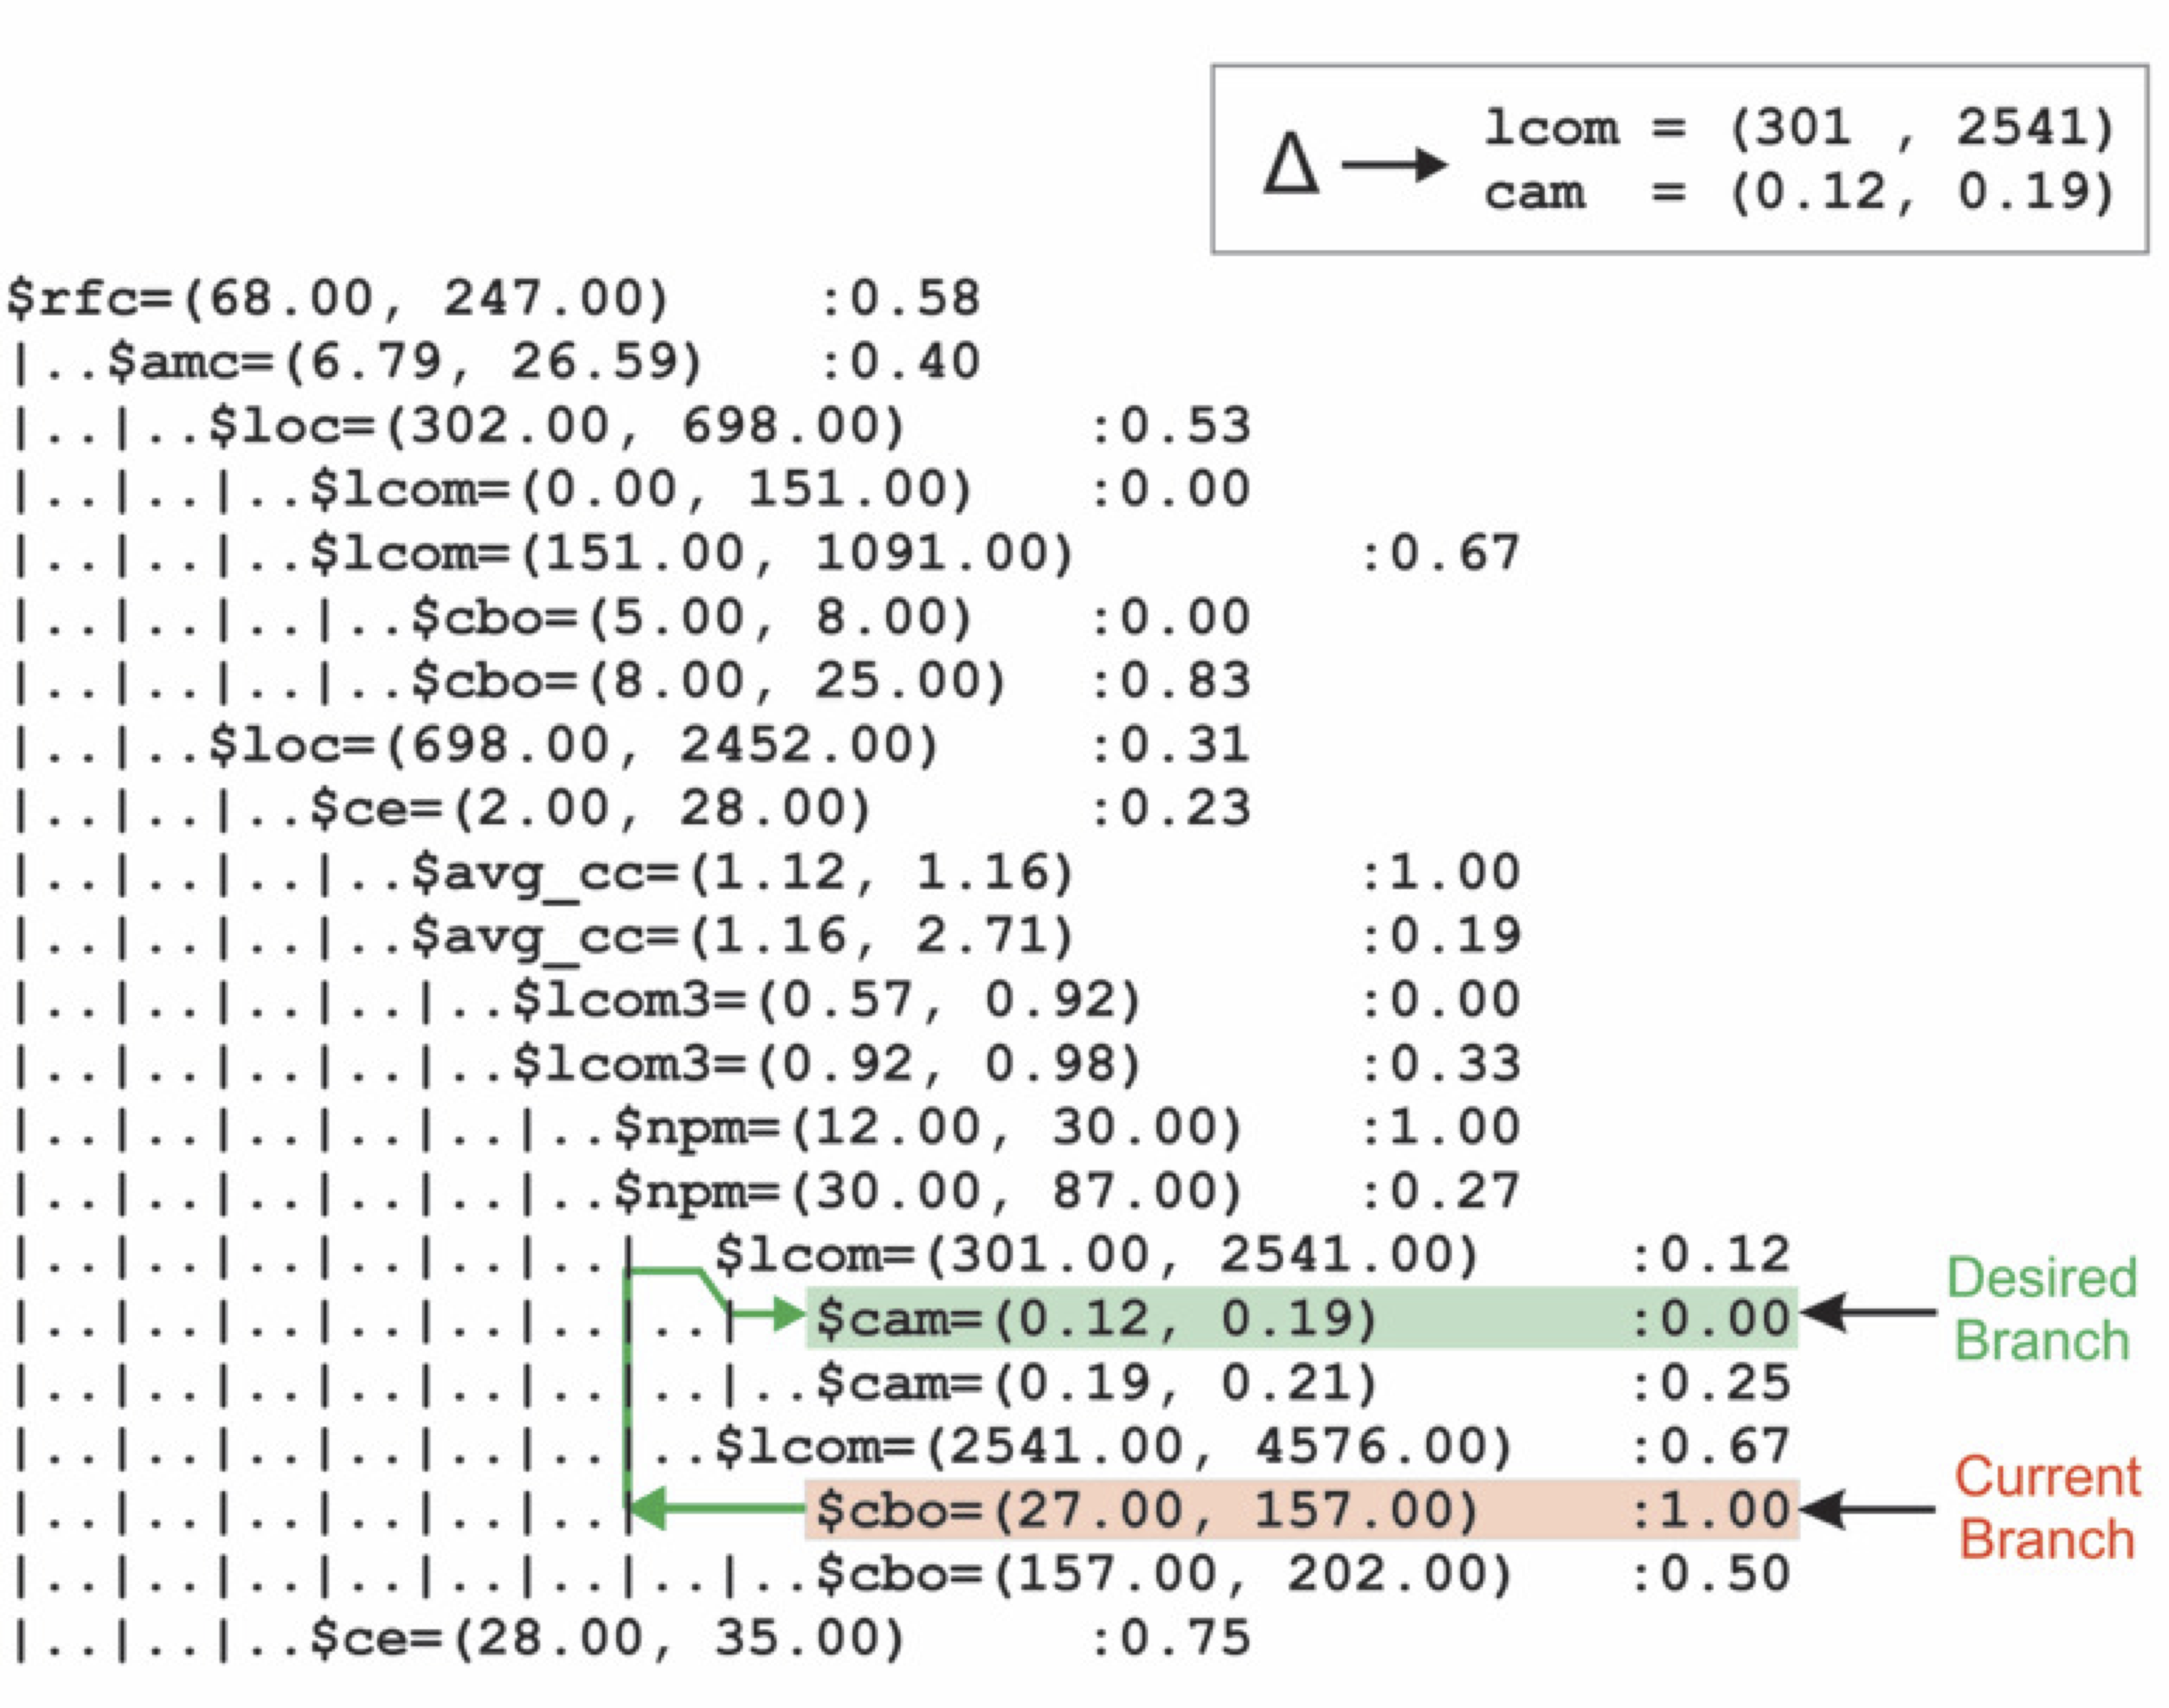
\includegraphics[width=0.99\linewidth]{XTREE_samp.png}
\end{minipage}\bigstrut\vspace{0.1cm}\\\hline
\end{tabular}}
\caption{Generating thresholds using XTREE.}\label{fig:xtree}
\end{figure}